% CREATED BY DAVID FRISK, 2016
\chapter{Toolbox}
I am working with AI Habitat, a simulation platform for working with embodied AI\cite{habitat19iccv}. It consists of two parts, Habitat-Sim, the 3D simulator, and Habitat-Lab, the library for embodied AI development. 

\subsection{The Model}
\label{subsection:model}
I am starting with the Embodied Question Answering baseline in Habitat-Lab, which consists of three parts, a CNN for initial feature extraction, a navigation module, called PACMAN, and a question answering module\cite{embodiedqa}.
The CNN feature extractor is trained on three tasks: RGB reconstruction, semantic segmentation, and depth estimation.
The navigation is trained to imitate shortest path navigation. % SD 2021-05-01 15:07:05 +0200: Imitation learning here is used to distinguish it from reinforcement learning. However, in my underastanding, imitation elarning is just standard ML.
The question answering module is given the last five frames of navigation (in training taken during ground-truth shortest path navigation, where a frame is the view the agent has after taking an action), and then predicts an answer from a set of possible answers. 
The training of the Habitat-Lab version of the model\footnote{available here: \url{https://github.com/facebookresearch/habitat-lab/tree/master/habitat_baselines/il}} differs somewhat to the version presented in the Embodied Question Answering paper\cite{embodiedqa}. For the original model, the CNN, question answering, and navigation modules were all trained separately, and then reinforcement learning was used to fine-tune, and more strongly link the question answering and navigation modules, by using accurate question answering % SD 2021-05-01 15:13:19 +0200: the success of, i.e. yes/no but no more information than this
% NI 2021-05-17: do not forget to note that only the navigation was fine-tuned through RL, the question answering has been frozen (section 4.1 in the paper)
as part of the reward for the navigation module. This reinforcement learning is missing from the habitat version of the model; the components of the model are only trained separately. 

% SD 2021-05-01 15:14:03 +0200: Reference to the Habitat-Lab github. Reverse the order of descriptions: navigation before QA

% SD 2021-05-01 15:21:10 +0200: Here it would be in place to include a model diagram and then indicate in what ways the baseline model is different from the original Das paper. Later on you can use modified version of the same diagram to point our your extensions. It would also be good to mention the paramateres of the model, i.e. the sizes of inputs, outputs and the intermediate layers.


\section{The Datasets}
% SD 2021-05-01 15:15:54 +0200: Present tense is okay since this a description of the current research; normally we would use past tense to distinguish what we are doing here from the previous publication.
I am using the Matterport3D dataset, a dataset of real interiors with human annotation of objects, as my scene dataset\cite{matterport}. 
I am using the MP3D-EQA task dataset, which was created using code to automatically generate questions and answers to correspond with annotated scenes in the Matterport3D dataset\footnote{The dataset is available in the habitat-lab repository here: \url{https://github.com/facebookresearch/habitat-lab/#data}}\cite{eqa_matterport}. 

% SD 2021-05-01 15:14:59 +0200: Reference to git repository.

\subsection{Interiors}

\subsection{MP3D-EQA Dataset} 
This dataset contains questions of three types: 'color\_room': \emph{What color is the <obj> in the <room>?}, 'color': \emph{What color is the <obj>?}, and 'location': \emph{What room is the <obj> located in?}. This dataset was based off of the EQA-V1 dataset, which was developed by Das et al and used in the development of the EQA model described above\footnote{Code for generating EQA-V1 questions is available here: \url{https://github.com/facebookresearch/EmbodiedQA}}\cite{embodiedqa}. There were some differences between the datasets, however. The EQA-V1 dataset included a fourth type of question, prepositional questions: \emph{What is <on/above/below/next to? the <obj> in the <room>?}, but these are not present in MP3D-EQA. They were removed because a limited number were generated, and those had strong biases. % SD 2021-05-01 15:17:33 +0200: I'm not sure if I udnerstand. One can create relations between any two objects. 
EQA-V1 was built based on the SUNCG scene dataset, which is no longer available, due to a legal dispute\cite{planner5d}. % SD 2021-05-01 15:18:04 +0200: Mention earlier that this was used in the original paper. 

The dataset has the most 'color\_room' questions, as shown in Tab.~\ref{tab:q_breakdown}.

\begin{table}[h]
\centering
\caption{Question Type Breakdown}
\begin{tabular}{ |l|l|l| }
\hline
\textbf{question type} & \textbf{percentage of training set} & \textbf{percentage of evaluation set} \\
\hline
color\_room & 69.85908 & 68.46154\\
color & 15.91858 & 17.69231\\
location & 14.22234 & 13.84615\\
\hline
\end{tabular}
\label{tab:q_breakdown}
\end{table}

The dataset has a fixed train/eval split. There is one object which only occurs in the evaluation set ('toaster'), and one answer that only occurs in the evaluation set ('gym'). More details about the answers can be found in Appendix~\ref{app:answercounts}.

\subsubsection{Limitations}
The paper which introduces the MP3D-EQA dataset was mainly focused on the navigation aspect of the task, and the question types reflect that. A color or location question should theoretically be a good indication of whether or not the agent has successfully navigated to the object, but actually answering the question may not require as complex of reasoning, in that it shouldn't require a long memory to answer. \newline
However, color identification is actually a very difficult task. One issue is purely visual--an object's color looks different in different lighting conditions, so someone might see something as light grey in good light, but in dimmer light only see it as grey. Another, more complex issue, is related to language: the way that humans identify and refer to colors is context dependent. Monroe et al created a dataset of color descriptions using pairs of Amazon Mechanical Turk participants\cite{colorsincontext}. One member of the pair was the speaker, the other was the listener. Both people could see the same three color samples, and the speaker was given one of them as the 'target', which they needed to convey to the listener. There were three possible situations: baseline, or 'far', where all three samples were very distinct, such as pink, green, and yellow; split, where one of the other colors (called distractors) was close to the target, such as two shades of blue, and then the last distractor was far, for example yellow; and close, where both distractors were similar to the target (all shades of blue, for example). They found that in the 'split' and 'close' conditions, the speaker used more comparatives (t.ex: lighter blue) and superlatives (t.ex: the lightest one), and also was more likely to use 'high specificity' color terms, such as 'magenta' or 'teal', using more basic terms, such as 'red' or 'blue', in the 'far' condition. This suggests that people would adjust their descriptions of an object's color based on what is around it. Another color issue, specific to this dataset, is that the colors used for annotation (done by Amazon Mechanical Turk workers), come from Kenneth L. Kelly's 'Twenty-two colors of maximum contrast', with the addition of 'off-white' and 'slate grey', since they are very common in indoor scenes\cite{kellycolors}. However, Kelly's colors were not designed to be natural color descriptions; they were developed as a set of colors that could be used in situations where contrast was needed--for example color coding of graphs. This is shown by the inclusion of both 'buff' and 'yellowish pink' in the color set. Off-white and white are also prone to being confused due to lighting conditions.\newline

The dataset of questions and answers for EQA in Habitat was automatically generated, and may contain some errors. One example of this is shown in Fig.~\ref{fig:err_ex}, in which the VQA model answered that the sofa in the living room is tan, but the ground truth answer is that it is yellow. However, looking at the image, I see a tan sofa and a yellow armchair. It seems that at some point, the armchair was annotated as a sofa, but the model is identifying the tan sofa as the sofa being asked about. 

\begin{figure}[h]
	\centering
	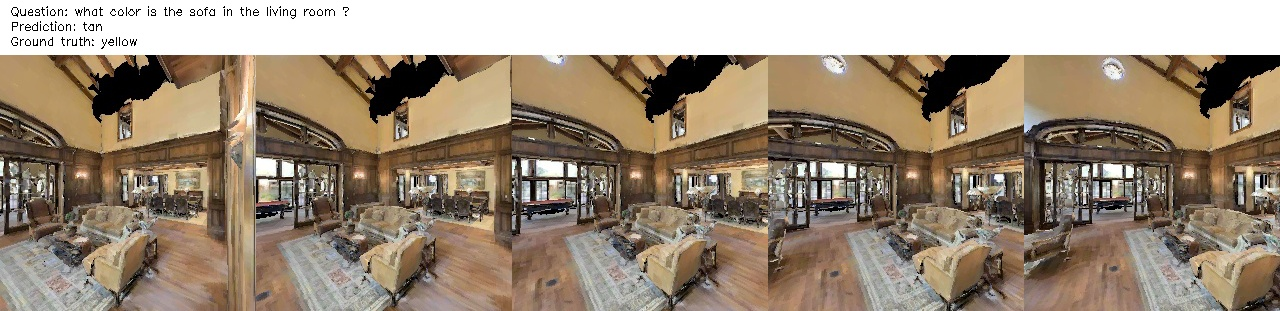
\includegraphics[width=\textwidth]{./figure/error_images/ckpt_0_121_image.jpg}
	\caption{Error Example}
	\label{fig:err_ex}
\end{figure}


% SD 2021-05-01 15:31:45 +0200: The following text should go into a separate section which would be describing our research questions and the experiments to answer them: a good way of doing this is to direct the discussion in the previous secitons in such a way that a reader would have a clear idea what the open questions are (directed by you of course) so that your research questions follow naturally.


